\section{Benchmarking} \label{benchmarking}
We used datasets of 2 different sizes to perform the benchmarking of the
application. Table \ref{tab:datasets} shows the details of the two datasets.
The CreateWord2VecModel spark application is most complex and time
consuming application. We used this application for the benchmarking. We
deployed the application on Chameleon cloud and Jetstream cloud. Table
\ref{tab:cloudconfig} shows the details for the cluster configurations on
Chameleon and Jetstream clouds.

\begin{table}[htbp]
\centering
\caption{\bf Dataset Used for Performance Measurement}
  \begin{tabular}{l|c|r}
    \hline
    Parameter & Dataset1 & Dataset2 \\
    Size of crawldb & 1.4MB & 7.4MB \\
    Count of files in crawldb & 100 & 500 \\
    Source & Wikipedia & Wikipedia \\
    \hline
  \end{tabular}
  \label{tab:datasets}
\end{table}


\begin{table}[htbp]
\centering
\caption{\bf Dataset Used for Performance Measurement}
  \begin{tabular}{ l | c | r }
    \hline
    Parameter & Chameleon Cluster & Jetstream Cluster \\
    Cluster name & cluster-005 & cluster-010 \\
    Nodes & 2 & 2 \\
    OS & Ubuntu 14.04 & Ubuntu 14.04 \\
    Flavor & m1.medium & m1.medium \\
    Secgroup & default & default \\
    Assign floating IP & True & True \\
    Cloud & chameleon & iujetstream \\
    \hline
  \end{tabular}
  \label{tab:cloudconfig}
\end{table}


Figure \ref{fig:compare147} shows the total time taken by CreateWord2Vec
application for Dataset1 on the Chameleon and Jetstream cloud environments.
\begin{figure}[htbp]
\centering
\fbox{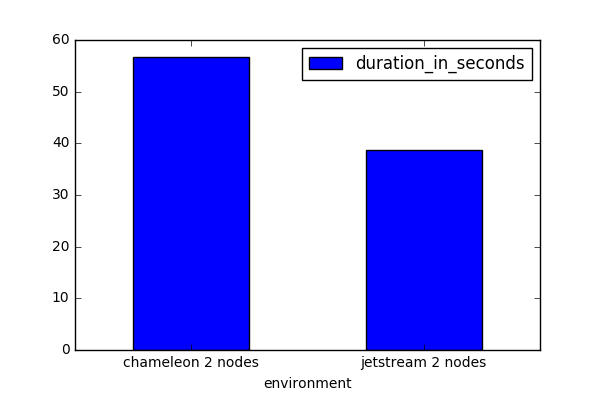
\includegraphics[width=\linewidth]{images/compare147.png}}
\caption{Time taken by CreateWord2Vec for Dataset1}
\label{fig:compare147}
\end{figure}

Figure \ref{fig:compare522} shows the total time taken by CreateWord2Vec
application for Dataset2 on the Chameleon and Jetstream cloud environments.
\begin{figure}[htbp]
\centering
\fbox{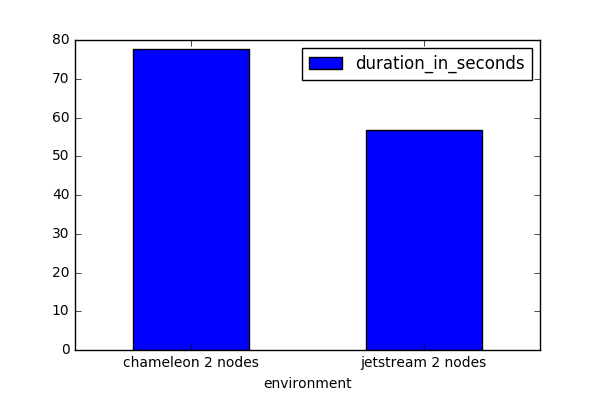
\includegraphics[width=\linewidth]{images/compare522.png}}
\caption{Time taken by CreateWord2Vec for Dataset2}
\label{fig:compare522}
\end{figure}

\subsection{Working with large dataset} \label{benchmarklargedatasets}
There are several configuration parameters added in the application to
fine tune the behavior of the spark applications. When working with larger
datasets, the spark applications can go out of memory. Following parameters
can be configured in the config.propertise to handle such situation.

\begin{verbatim}
spark_executor_memory = <memory given to executor>
spark_driver_memory = <memory given to driver>
max_result_size = <maximum result size>
\end{verbatim}

